% This file was created with tikzplotlib v0.10.1.
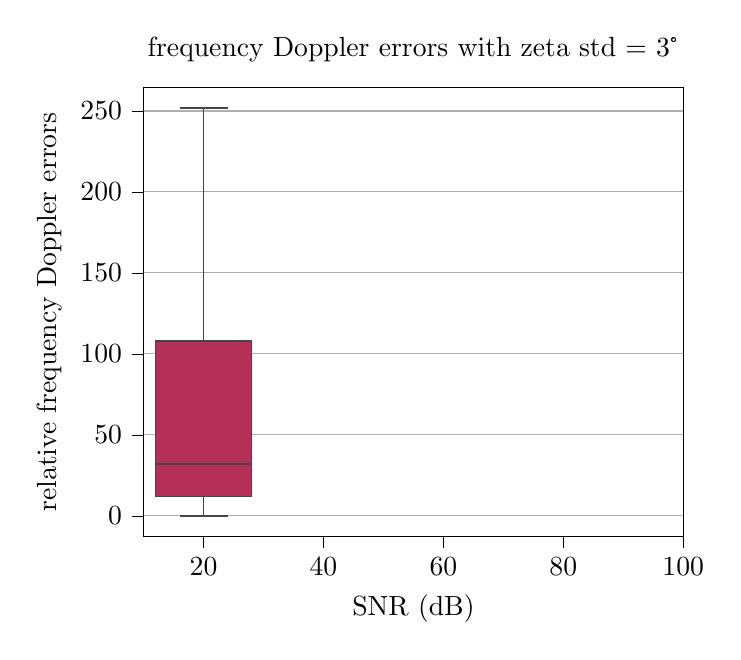
\begin{tikzpicture}

\definecolor{brown1814888}{RGB}{181,48,88}
\definecolor{darkgray176}{RGB}{176,176,176}
\definecolor{darkslategray69}{RGB}{69,69,69}

\begin{axis}[
tick align=outside,
tick pos=left,
title={frequency Doppler errors with zeta std = 3°},
x grid style={darkgray176},
xlabel={SNR (dB)},
xmin=-0.5, xmax=4,
xtick style={color=black},
xtick={0,1,2,3,4},
xticklabels={20,40,60,80,100},
y grid style={darkgray176},
ylabel={relative frequency Doppler errors},
ymajorgrids,
ymin=-12.5834784887352, ymax=264.26095687957,
ytick style={color=black}
]
\path [draw=darkslategray69, fill=brown1814888, semithick]
(axis cs:-0.4,11.9965581091356)
--(axis cs:0.4,11.9965581091356)
--(axis cs:0.4,108.102502787571)
--(axis cs:-0.4,108.102502787571)
--(axis cs:-0.4,11.9965581091356)
--cycle;
\addplot [semithick, darkslategray69]
table {%
0 11.9965581091356
0 0.000359482551402834
};
\addplot [semithick, darkslategray69]
table {%
0 108.102502787571
0 251.677118908284
};
\addplot [semithick, darkslategray69]
table {%
-0.2 0.000359482551402834
0.2 0.000359482551402834
};
\addplot [semithick, darkslategray69]
table {%
-0.2 251.677118908284
0.2 251.677118908284
};
\addplot [semithick, darkslategray69]
table {%
-0.4 32.0622182058469
0.4 32.0622182058469
};
\end{axis}

\end{tikzpicture}
